\section{Multilayer perceptron}


Dans cet  exercice, nous devons impl�menter un r�seau des neurones. Pour faire cela, on doit indiquer le nombre d'entr�es des features, le nombre des neurones pr�sents dans la couche cach� et le nombre des sorties. Ensuite, il a fallu mettre en place le backpropagatoin trainer \texttt{BackProrpTraing} qui s'occupe d'entrainer notre r�seau de neurones avec le dataset de trainining et deux param�tres: \texttt{momentum} et le \texttt{learning rate}. Pour commencer l'entrainement du r�seau de neurones, on appelle ensuite \texttt{trainer.train()} qui ex�cute une \texttt{�poque} d'entrainement sur le r�seau de neurones. Voici donc le code de cet exercice :
\lstinputlisting{code/FNN.py}
\newpage


Avec l'entrainement par d�faut on a en r�sultat une \texttt{pr�cision de 0.55} un \texttt{recall de 0.67} et un  \texttt{f-score de 0.60}.
La matrice de confusion de la figure \ref{mat001} nous montre aussi que les classes ne sont pas bien reconnues par le classificateur:
\begin{figure}[h]
  \centering
    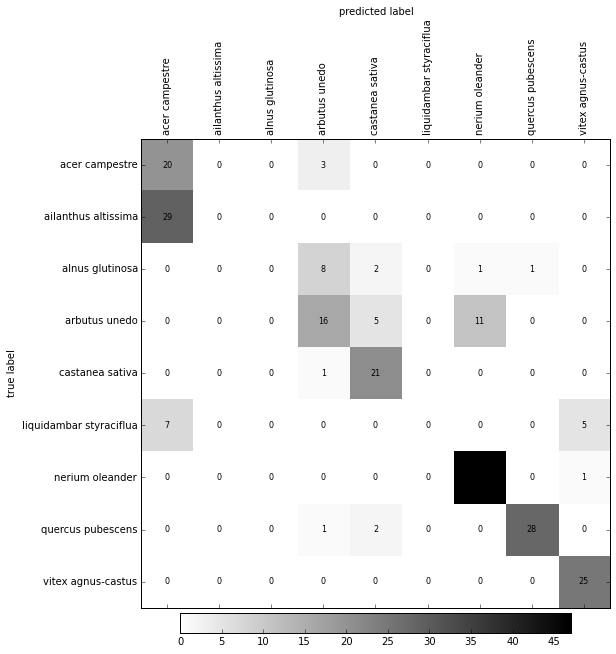
\includegraphics[width=0.6\linewidth]{img/mconf_001.png}
  \caption{Matrice de confusion avec learning rate 0.001 et 50 it�rations}
  \label{mat001}
\end{figure}
\newpage


On a d� donc tuner ces param�tres pour am�liorer les r�sultats. On a commenc� par modifier le training rate a \texttt{trainintrate=0.2} pour chercher d'am�liorer plus rapidement l'erreur g�n�r�e par le'entrainement et arriver a de meilleurs r�sultats. 


Par contre, comme on pou voire du graphique de la figure \ref{graph1} l'erreur d'entrainement est assez instable, cela n'est pas optimale pour trouver une bonne convergence. 
\begin{figure}[h]
  \centering
    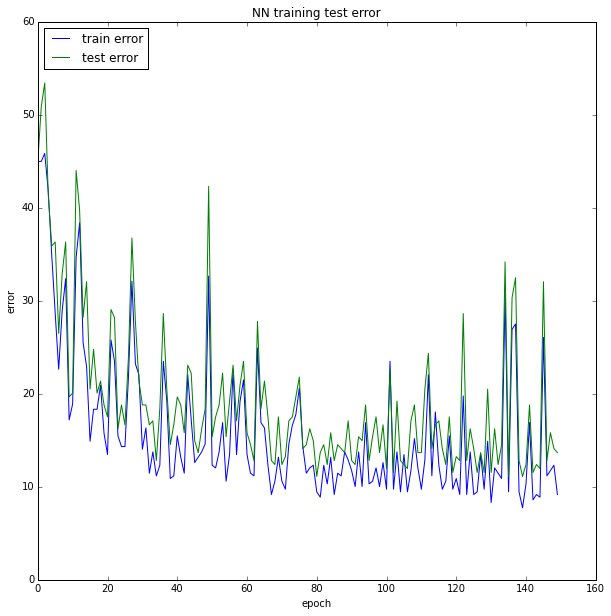
\includegraphics[width=0.6\linewidth]{img/graph3.png}
  \caption{Erreur d'entrainement et de test}
  \label{graph1}
\end{figure}
\newpage


Nous avons donc essay� plusieurs param�tres et en final on a trouv� certains qui parait le meilleurs. 
En final on a ex�cut� \texttt{150 it�rations} avec un \texttt{momentum=0.1} et le \texttt{learningrate=0.03}.On a eu en r�sultat une \texttt{precision de 0.82} un \texttt{recall de 0.86} et un  \texttt{f-score de 0.84} que sont assez similaire au r�sultat du KNN.
Le graphique repr�sent� par la figure \ref{graph003} nous montre que l'entrainement est plus stable qu? avant et qu? on arrive a la convergence. On pourra en effet m�me diminuer le nombre d'it�rations.
\begin{figure}[h]
  \centering
    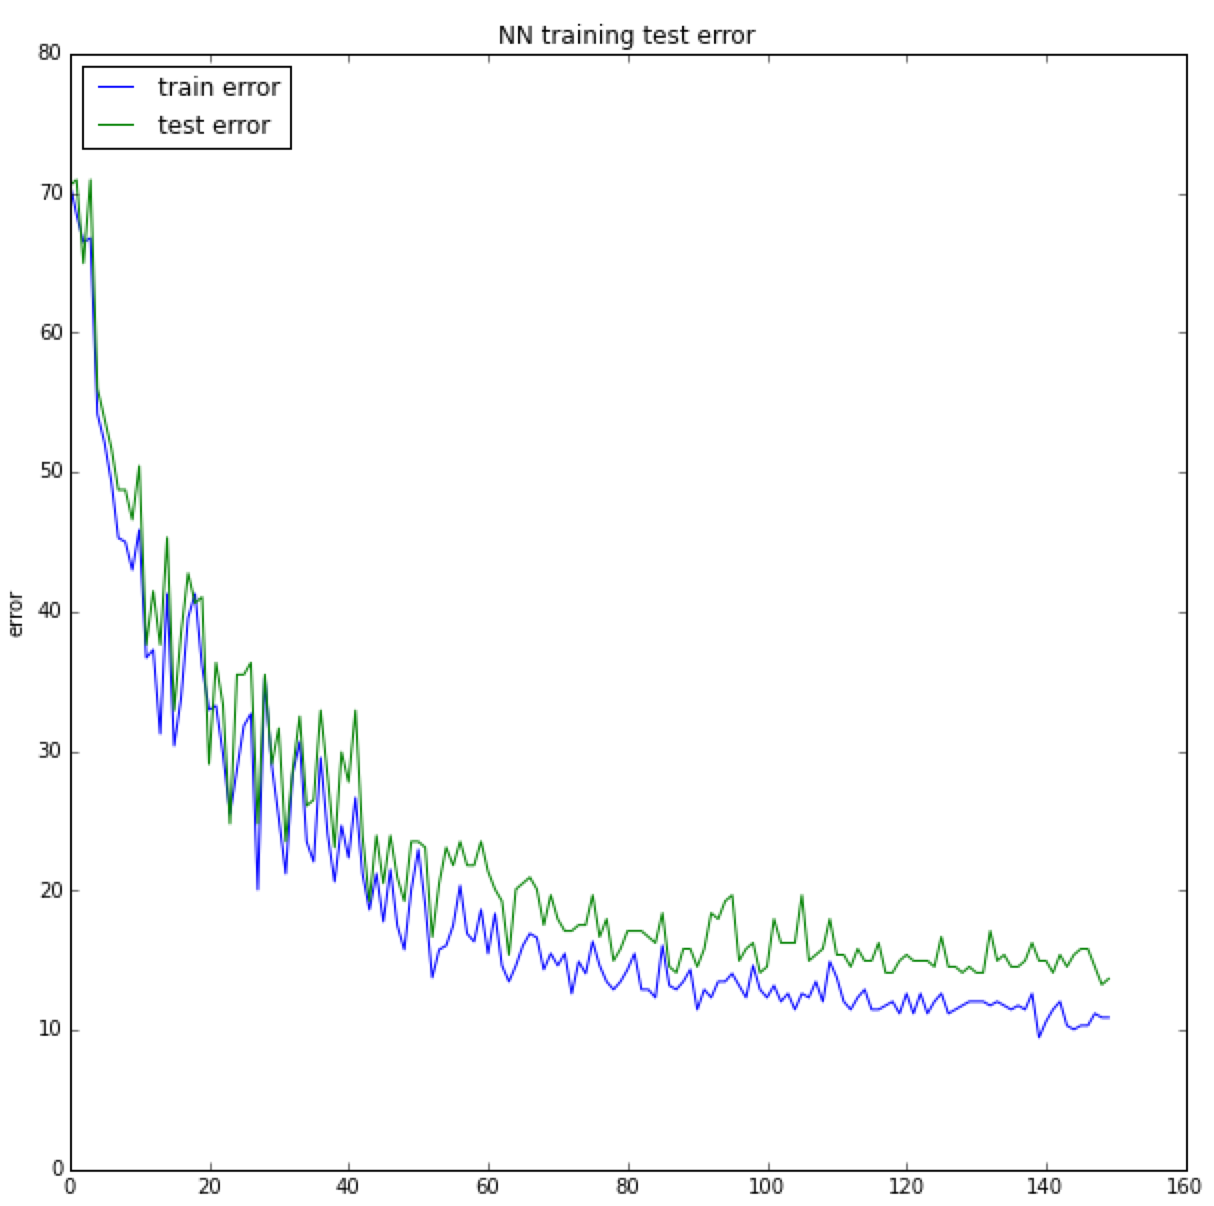
\includegraphics[width=0.6\linewidth]{img/graph003.png}
  \caption{Erreur d'entrainement et de test avec \texttt{training\_rate=0.003}}
  \label{graph003}
\end{figure}
\newpage
En final la matrice de la figure \ref{maconf003} nous montre que les classes sont beaucoup mieux class�es qu? avant et que mis � part la la classe \texttt{liquidambar styraciflue}, sont suffisamment bien reconnu par le classificateur.

\begin{figure}[h]
  \centering
    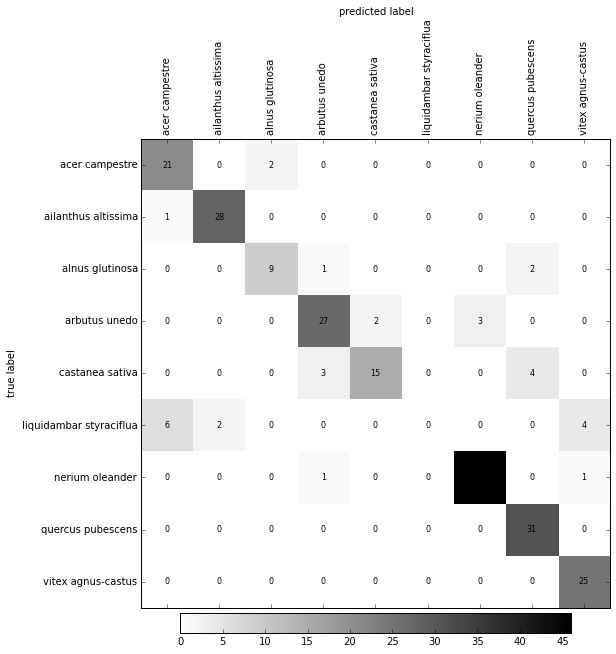
\includegraphics[width=0.6\linewidth]{img/mconf_003.png}
  \caption{Matrice de confusion finale}
  \label{mconf003}
\end{figure}



